\subsubsection{Model podstawowy}

\begin{figure}[ht]
	\centering
	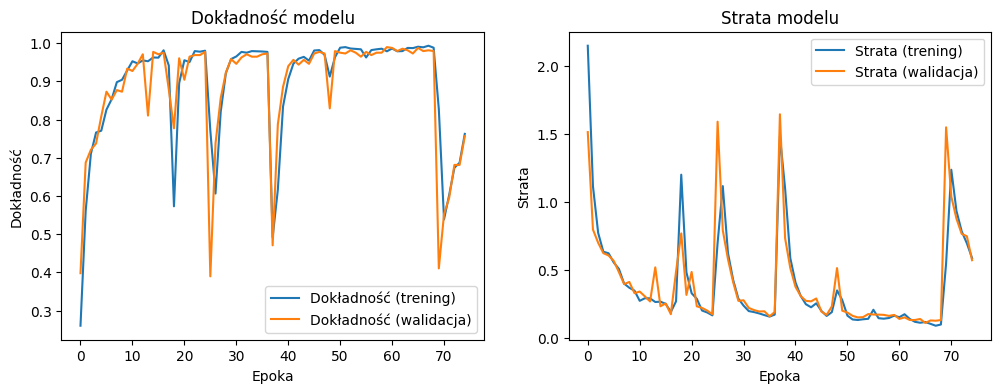
\includegraphics[height=5.5cm]{partials/tests/images/v2_epoch75.png}
	\caption{Wyniki testów dla modelu podstawowego}
	\label{Fig:tests-base-1}
\end{figure}
\FloatBarrier

\begin{figure}[ht]
	\centering
	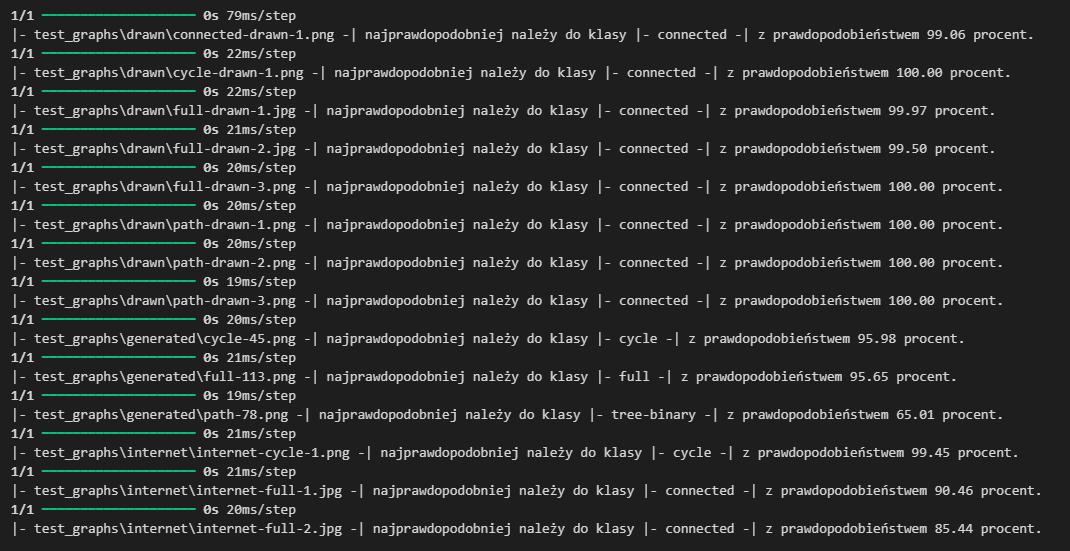
\includegraphics[height=7cm]{partials/tests/images/v2_epoch75_img_tests.png}
	\caption{Klasyfikacja obrazów zewnętrznych dla modelu ze zmienną liczbą wierzchołków}
	\label{Fig:tests-base-2}
\end{figure}
\FloatBarrier

\subsubsection{Model z walidacją krzyżową}

W przypadku standardowego modelu z walidacją krzyżową model bardzo szybko uległ przeuczeniu.
Już po szóstej iteracji dokładność na zbiorze walidaycjnym wyniosła 100\%, co nie jest realistycznie możliwe.
Została podjęta próba ograniczenia przeuczenia poprzez zwiększenie zbioru danych, zmiany liczby epok w modelu
oraz manipulacji współczynnikami dropout i regularyzacji.
W każdym przypadku model zwracał niezadowalające wyniki wynoszące 100\% po jednej z początkowych iteracji.

\begin{figure}[ht]
	\centering
	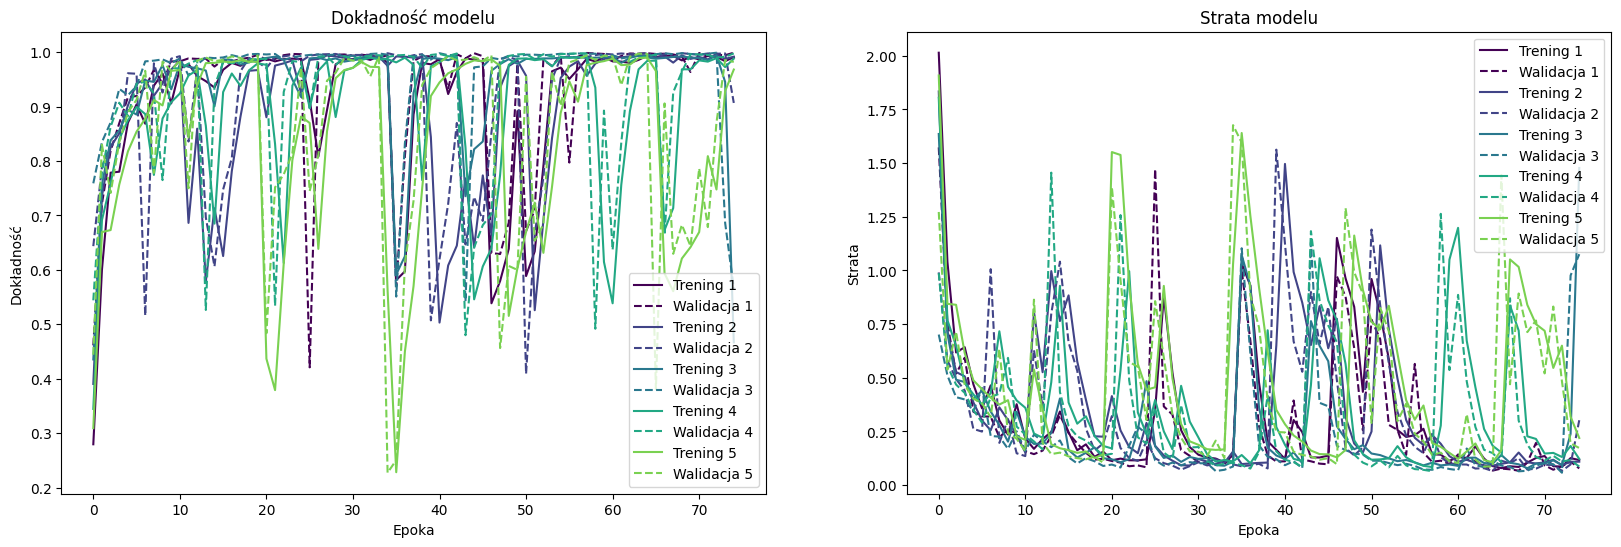
\includegraphics[height=5.5cm]{partials/tests/images/v2_crossvalid.png}
	\caption{Wyniki testów dla modelu z walidacją krzyżową}
	\label{Fig:tests-cv-1}
\end{figure}
\FloatBarrier

Z powodu przeuczenia model nie radził sobie z zewnętrznymi obrazkami testowymi.
Większość grafów określił jako grafy pełne, co nie jest zgodne ze stanem rzeczywistym.

\begin{figure}[ht]
	\centering
	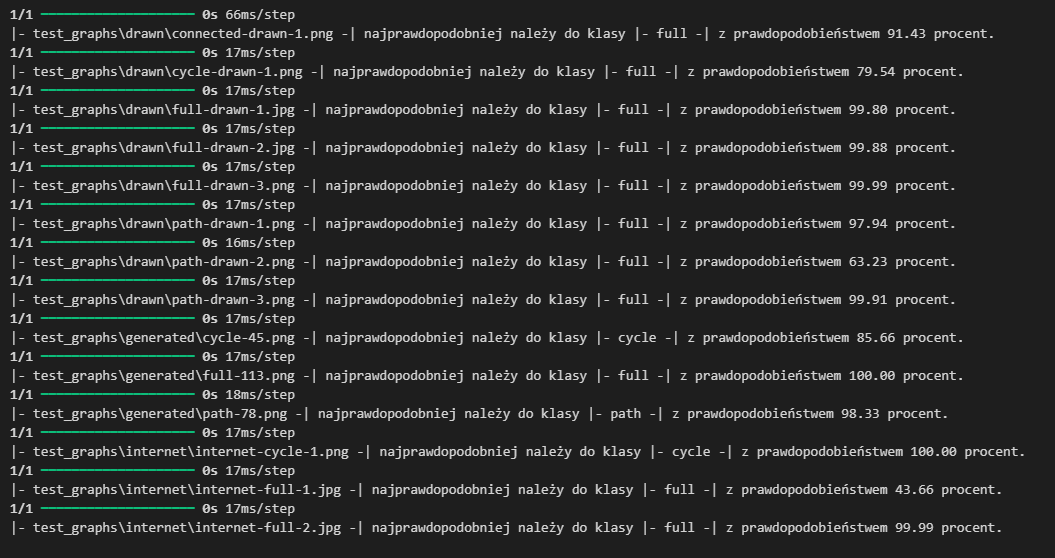
\includegraphics[height=7cm]{partials/tests/images/v2_crossvalid_img_tests.png}
	\caption{Klasyfikacja obrazów zewnętrznych dla modelu z walidacją krzyżową}
	\label{Fig:tests-cv-2}
\end{figure}
\FloatBarrier

\subsubsection{Model ze zmienną liczbą wierzchołków}
Najlepsze wyniki pod względem rozpoznawania zewnętrznych obrazków testowych
oraz realistycznej dokładności na zbiorze walidacyjnym,
zostały uzyskane przy użyciu modelu sieci neuronowej uczonej na rysunkach grafów z różną liczbą wierzchołków.
Było to odpowiednio 4, 5, 6 oraz 7 wierzchołków.

\begin{figure}[ht]
	\centering
	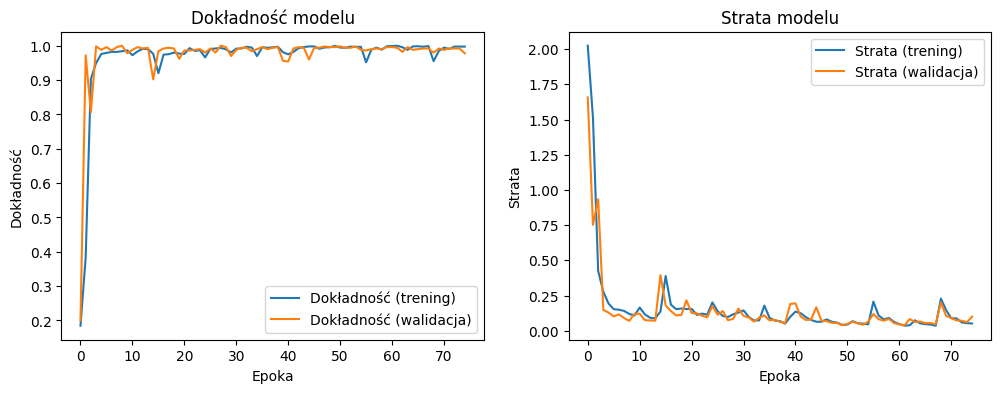
\includegraphics[height=5.5cm]{partials/tests/images/v2_multiple_edges_epoch75.png}
	\caption{Wyniki testów dla modelu ze zmienną liczbą wierzchołków}
	\label{Fig:tests-var-1}
\end{figure}
\FloatBarrier

Model nie poradził sobie zbyt dobrze z obrazami zewnętrznymi, lecz znacznie lepiej niż model z walidacją krzyżową.
Poprawnie wskazanych klas grafów było 5 z 14 wszystkich rysunków.
Mimo, że model jest w stanie poprawnie określić niektóre typy grafów poprawnie,
wciąż jest to dokładność niższa niż 50\%.

\begin{figure}[ht]
	\centering
	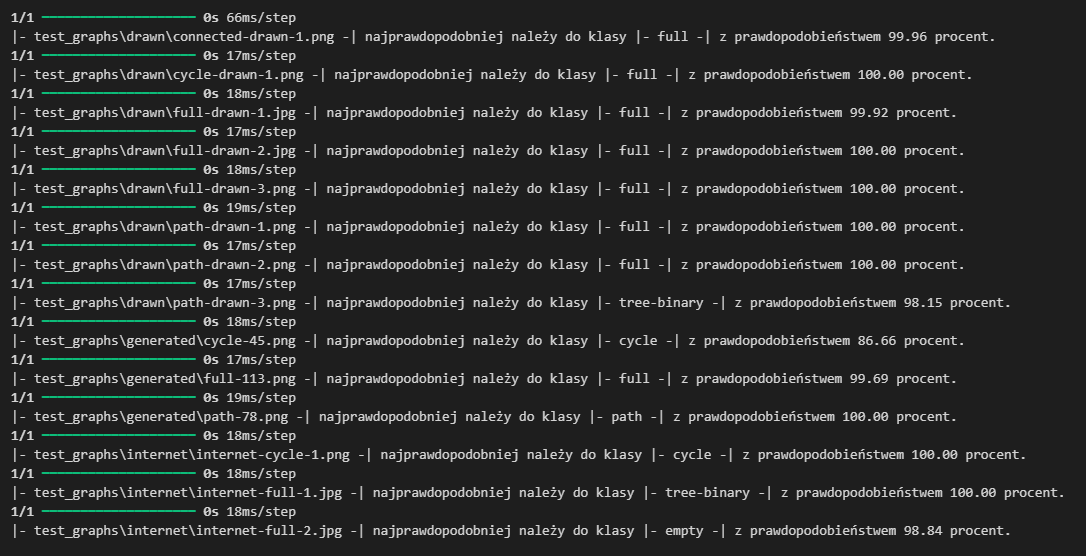
\includegraphics[height=7cm]{partials/tests/images/v2_multiple_edges_epoch75_img_tests.png}
	\caption{Klasyfikacja obrazów zewnętrznych dla modelu z walidacją krzyżową}
	\label{Fig:tests-var-2}
\end{figure}
\FloatBarrier

\subsubsection{Model ze zmienną liczbą wierzchołków i walidacją krzyżową}

\begin{figure}[ht]
	\centering
	% \includegraphics[height=5.5cm]{partials/tests/images/v2_multiple_edges_crossvalid.png}
	\caption{Wyniki testów dla modelu ze zmienną liczbą wierzchołków i walidacją krzyżową}
	\label{Fig:tests-csvar-1}
\end{figure}
\FloatBarrier

\begin{figure}[ht]
	\centering
	% \includegraphics[height=5.5cm]{partials/tests/images/v2_multiple_edges_crossvalid_img_tests.png}
	\caption{Klasyfikacja obrazów zewnętrznych dla modelu ze zmienną liczbą wierzchołków i walidacją krzyżową}
	\label{Fig:tests-csvar-2}
\end{figure}
\FloatBarrier